\chapter{Reduced Problem}

\section{Definition}

While there are several classes of WEC technology currently under development, for example (see \cite{Zhang_2021})

\begin{enumerate}
	\item point absorbers (like the AquaBuoy WEC)
	\item attenuators (like the Pelamis WEC)
	\item terminators (like the Oyster WEC)
	\item oscillating water columns (like the Mutriku WEC)
	\item overtopping devices (like the Wave Dragon WEC)
\end{enumerate}

\noindent the point absorber class appears to be emerging as a particularly promising candidate. As such, this work will focus exclusively on this class of tech. \par 
That said, consider a point absorber WEC which is a cylindrical float riding a bottom-fixed piling as illustrated in Figure \ref{fig:WEC_reduced_problem}.\footnote{Think a WEC design which is intended to be installed at the waterline of existing offshore infrastructure, like wind turbines or oil rigs.}

\begin{figure}[H]
    \centering
    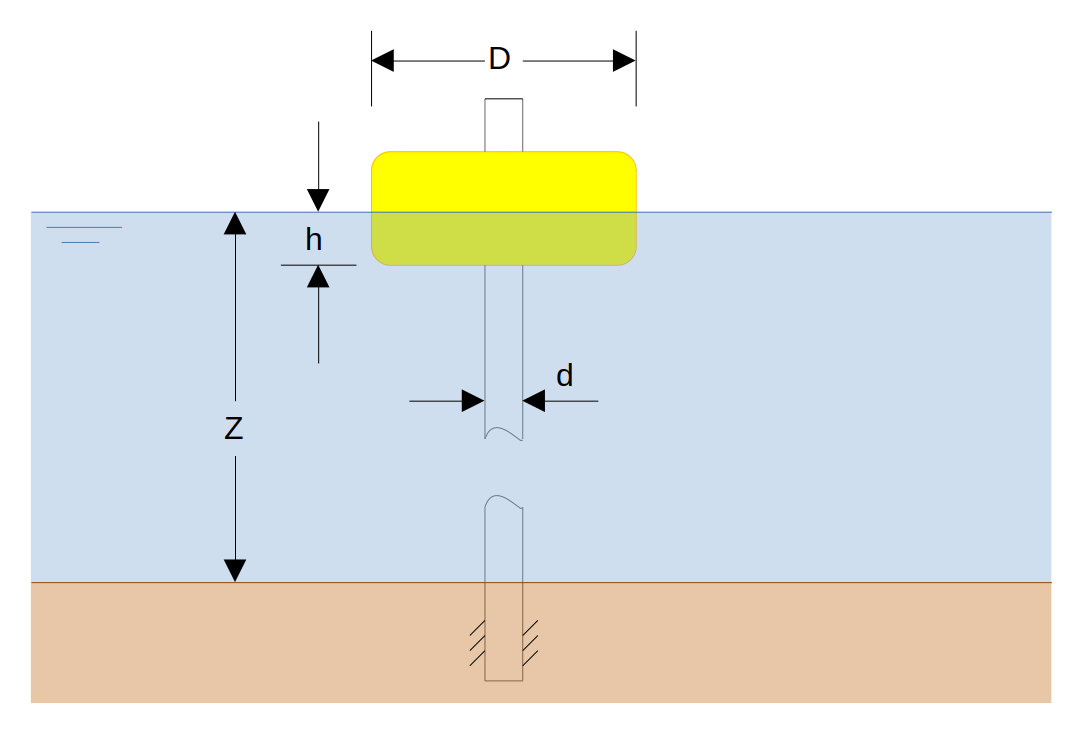
\includegraphics[width=1\textwidth]{WEC/WEC_zero_sea_equilibrium.png}
    \caption{A point absorber as a cylindrical float riding a bottom-fixed piling.}
    \label{fig:WEC_reduced_problem}
\end{figure}

\noindent That is, a float of diameter $D>d$ and with resting draft $h>0$ is riding a bottom-fixed piling of diameter $d>0$ in a sea of depth $Z>0$. The basic operating principle here is that wave action causes the float to oscillate, and the relative motion between the float and piling can then drive some power takeoff device.

\section{Simplifying Assumptions}

To begin assembling the reduced problem, a number of simplifying assumptions are made; namely

\begin{enumerate}
	\item Inviscid fluid (i.e., no drag).
	\item Forces due to wave incidence, wave diffraction, and wave radiation are all negligible compared to buoyancy forces.
	\item Added mass effects can be ignored.
	\item Fluid memory effects can be ignored.
	\item Power takeoff (PTO) dynamics are linear.
	\item The WEC is heave constrained (i.e., it is a single degree-of-freedom system).
\end{enumerate}

\noindent As such, the only forces acting on the WEC in this reduced case are weight, buoyancy, and the reaction from the PTO. Furthermore, the WEC can only move in heave (i.e. up and down).

\section{Constructing the Differential Equation of Motion}

Consider the free-body diagram illustrated in Figure \ref{fig:WEC_free_body}.

\begin{figure}[H]
    \centering
    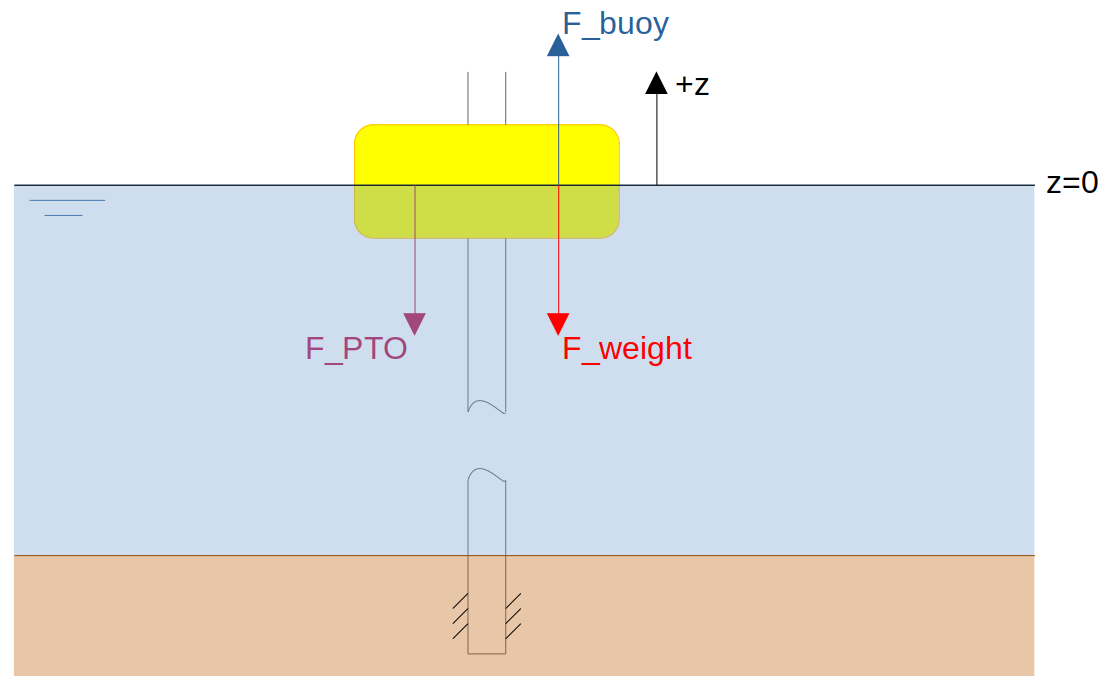
\includegraphics[width=1\textwidth]{WEC/WEC_free_body.png}
    \caption{Free-body diagram for the reduced WEC dynamics.}
    \label{fig:WEC_free_body}
\end{figure}

\noindent That is, define positive float motion ($+z$) as upward, and define the origin ($z=0$) as the mean sea level. Therefore, for positive float motion, the driving buoyancy force has positive orientation and the PTO reaction has negative orientation. Of course, weight always has negative orientation in this case.\par 
As per Newton's Second Law (Newton II), the sum of external forces acting on a body is equal to the time rate-of-change of the body's momentum. So, in this case, application of Newton II yields

\begin{equation}
	F_\textrm{buoy} + F_\textrm{weight} + F_\textrm{PTO} = \frac{d}{dt}\left\{m\dot{z}\right\}
	\label{eqn:Newton_II}
\end{equation}

\noindent Assuming a constant float mass $m>0$, it then follows that

\begin{equation}
	F_\textrm{buoy} + F_\textrm{weight} + F_\textrm{PTO} = m\ddot{z}
	\label{eqn:Newton_II_constant_mass}
\end{equation}

Now, the force due to weight is given simply by the product of float mass $m$ and acceleration due to gravity $g$; namely

\begin{equation}
	F_\textrm{weight} = -mg
	\label{eqn:float_weight}
\end{equation}

\noindent As for the reaction from the PTO, if one assumes constant stiffness and damping values $k\geq 0$ and $b\geq 0$ respectively, then it follows that

\begin{equation}
	F_\textrm{PTO} = -kz - b\dot{z}
	\label{eqn:PTO_reaction}
\end{equation}

\noindent Finally, the driving buoyancy force can be obtained by way of Archimedes' Principle, which states that a floating body experiences an upward buoyancy force equal to the weight of the fluid displaced. Therefore, for a float with a resting draft of $h$ in a fluid of density $\rho>0$, it follows in this case that

\begin{equation}
	F_\textrm{buoy} = \frac{\pi\rho g}{4}(D^2 - d^2)(h + \overline{\eta} - z)\quad\textrm{for}\quad h + \overline{\eta} - z \geq 0
	\label{eqn:buoyancy_force}
\end{equation}

\noindent where $\overline{\eta}$ is the deviation in sea surface elevation, from $z=0$, averaged over the waterplane area of the float. But then, the fact that the float has a resting draft of $h$ implies (again, by Archimedes) that

\begin{equation}
	m = \frac{\pi\rho h}{4}(D^2 - d^2)
	\label{eqn:float_mass}
\end{equation}

\noindent as this ensures that (\ref{eqn:float_weight}) and (\ref{eqn:buoyancy_force}) are equal and opposite when the system is at rest (i.e., $z=\dot{z}=\ddot{z}=0$ and $\overline{\eta}=0$), as one might logically expect. From this, it follows that

\begin{equation}
	F_\textrm{weight} = -\frac{\pi\rho gh}{4}(D^2 - d^2)
	\label{eqn:float_weight_Archimedes}
\end{equation}
 
Finally, substituting (\ref{eqn:PTO_reaction}) - (\ref{eqn:float_weight_Archimedes}) into (\ref{eqn:Newton_II_constant_mass}) and re-arranging yields (after simplifying) the following differential equation of motion 

\begin{equation}
	m\ddot{z} + b\dot{z} + \left(k + k_D\right)z = k_D\overline{\eta}\quad\textrm{for}\quad h + \overline{\eta} - z \geq 0
	\label{eqn:ODE}
\end{equation}

\noindent with

\begin{equation}
	k_D = \frac{\pi\rho g}{4}(D^2 - d^2)
	\label{eqn:k_D}
\end{equation}

\noindent Note that (\ref{eqn:ODE}) is a linear, second-order, ordinary differential equation with constant coefficients (and as such, can be solved exactly using classical methods).

\section{Solving the Differential Equation of Motion}

\subsection{General Solution to the Homogeneous Equation}

First, a general solution to the homogeneous equation is sought. That is, determine $z(t)$ such that

\begin{equation}
	m\ddot{z} + b\dot{z} + \left(k + k_D\right)z = 0
	\label{eqn:ODE_homogeneous}
\end{equation}

\noindent The classical approach here is by way of the trial solution

\begin{equation}
	z(t) = C\exp[rt]
	\label{eqn:homogeneous_trial_solution}
\end{equation}

\noindent Substitution of (\ref{eqn:homogeneous_trial_solution}) into (\ref{eqn:ODE_homogeneous}) then yields the second-order characteristic equation (in $r$), which in turn then leads to the general solution

\begin{equation}
	z(t) = C_1\exp\left[\frac{1}{2m}\left(-b+\sqrt{b^2 - 4(k + k_D)m}\right)t\right] + C_2\exp\left[\frac{1}{2m}\left(-b-\sqrt{b^2 - 4(k + k_D)m}\right)t\right]
	\label{eqn:ODE_general_solution}
\end{equation}

\noindent where $C_1$ and $C_2$ are arbitrary constants (see \texttt{Maple/ODE\_general\_solution.mw}). That said, assuming zero initial conditions (i.e., $z(0) = \dot{z}(0) = 0$) leads to $C_1 = C_2 = 0$. This assumption is made in this work, and so the general solution is here omitted.

\subsection{Expressing Average Sea Surface Elevation}

Since the differential equation of motion has constant coefficients, it follows that a particular solution to the nonhomogeneous equation can be obtained by way of the method of undetermined coefficients. However, in order to do so, an appropriate expression for $\overline{\eta}$ must first be obtained.\par
As per \cite{Holthuijsen_2010}, the deviation in the sea surface elevation (from mean sea level) over an area of sea can be expressed as a cosine series (in polar form) as follows

\begin{equation}
	\eta(r,\theta,t) = \sum_{n=1}^\infty a_n\cos\left(\frac{2\pi nt}{T} - k_nr\cos(\psi_n - \theta) - \phi_n\right)
	\label{eqn:eta_polar}
\end{equation}

\noindent where $a_n$ is component amplitude, $T>0$ is some fundamental period, $k_n>0$ is component wave number, $\psi_n\in[-\pi,\pi]$ is component direction, and $\phi_n\in[-\pi,\pi]$ is component phase (random, with uniform distribution). Applying the trig identity

$$ \cos(\alpha - \beta) = \cos(\alpha)\cos(\beta) + \sin(\alpha)\sin(\beta) $$

\noindent then expands (\ref{eqn:eta_polar}) as follows

\begin{equation}
	\eta(r,\theta,t) = \sum_{n=1}^\infty a_n\left[\cos\left(\frac{2\pi nt}{T} - \phi_n\right)\cos(k_nr\cos(\psi_n - \theta)) + \sin\left(\frac{2\pi nt}{T} - \phi_n\right)\sin(k_nr\cos(\psi_n - \theta))\right]
	\label{eqn:eta_polar_expanded}
\end{equation}

Now, $\overline{\eta}$ was introduced as the deviation in the sea surface elevation (from mean sea level) averaged over the waterplane area of the float. That is

\begin{equation}
	\overline{\eta}(t) = \frac{1}{A_\textrm{water}}\iint_{A_\textrm{water}}\eta(r,\theta,t)dA
	\label{eqn:eta_overline_integral}
\end{equation}

\noindent where $A_\textrm{water}$ is the waterplane area of the float. For the case of the cylindrical float considered in this work, (\ref{eqn:eta_overline_integral}) can be expressed as

\begin{equation}
	\overline{\eta}(t) = \frac{4}{\pi(D^2-d^2)}\int_{0}^{2\pi}\int_{\frac{d}{2}}^{\frac{D}{2}}\eta(r,\theta,t)rdrd\theta
	\label{eqn:eta_overline_integral_expanded}
\end{equation}

\noindent Next, approximation using a \textit{finite} cosine series allows one to express (\ref{eqn:eta_overline_integral_expanded}), by way of substitution of (\ref{eqn:eta_polar_expanded}), as 

\begin{multline}
	\overline{\eta}(t) \cong \\
		\frac{4}{\pi(D^2-d^2)}\sum_{n=1}^N\left[a_n\cos\left(\frac{2\pi nt}{T} - \phi_n\right)\int_{0}^{2\pi}\int_{\frac{d}{2}}^{\frac{D}{2}}r\cos(k_nr\cos(\psi_n - \theta))drd\theta\right] +\\
		\frac{4}{\pi(D^2-d^2)}\sum_{n=1}^N\left[a_n\sin\left(\frac{2\pi nt}{T} - \phi_n\right)\int_{0}^{2\pi}\int_{\frac{d}{2}}^{\frac{D}{2}}r\sin(k_nr\cos(\psi_n - \theta))drd\theta\right] \\
	\label{eqn:eta_overline_sum_of_integrals}
\end{multline}

\noindent Unfortunately, the integrals in (\ref{eqn:eta_overline_sum_of_integrals}) defy exact solution,\footnote{To the best of the author's ability.} and so the best that can be done here is some partial and asymptotic analysis to get a sense of the nature of (\ref{eqn:eta_overline_sum_of_integrals}). That said, such results (luckily) are forthcoming.\par 
To begin, attempting to solve the integrals in (\ref{eqn:eta_overline_sum_of_integrals}) exactly yields the following partial results (see \texttt{Maple/eta\_overline\_integrals.mw}).

\begin{subequations}
	\begin{equation}
		\int_{0}^{2\pi}\int_{\frac{d}{2}}^{\frac{D}{2}}r\cos(k_nr\cos(\psi_n - \theta))drd\theta = \frac{1}{2k_n^2}\int_{0}^{2\pi}[\cdots]d\theta
	\end{equation}
	{}\\
	\begin{equation}
		\int_{0}^{2\pi}\int_{\frac{d}{2}}^{\frac{D}{2}}r\sin(k_nr\cos(\psi_n - \theta))drd\theta = -\frac{1}{2k_n^2}\int_{0}^{2\pi}[\cdots]d\theta
	\end{equation}
	\label{eqn:eta_overline_integrals_partial_solution}
\end{subequations}

\noindent So then, presumably the dimensionless term

\begin{equation}
	\Pi_{k_n} = k_n^2(D^2 - d^2)
	\label{eqn:kDd_dimensionless_term}
\end{equation}

\noindent is of significance in an exact solution to the integrals in (\ref{eqn:eta_overline_sum_of_integrals}).

\newpage 
Next, for the limiting case of $d=0$, it can be shown (see \texttt{Maple/eta\_overline\_integrals.mw}) that

\begin{subequations}
	\begin{equation}
		\lim_{D\to 0^+} \frac{4}{\pi D^2}\int_{0}^{2\pi}\int_{0}^{\frac{D}{2}}r\cos(k_nr\cos(\psi_n - \theta))drd\theta = 1
	\end{equation}
	{}\\
	\begin{equation}
		\lim_{D\to 0^+} \frac{4}{\pi D^2}\int_{0}^{2\pi}\int_{0}^{\frac{D}{2}}r\sin(k_nr\cos(\psi_n - \theta))drd\theta = 0
	\end{equation}
	\label{eqn:lim_D_0}
\end{subequations}

\noindent And so, as $D\to 0^+$ in this case,

\begin{equation}
	\lim_{D\to 0^+}\overline{\eta}(t)\cong\sum_{n=1}^N a_n\cos\left(\frac{2\pi nt}{T} - \phi_n\right)
	\label{eqn:eta_overline_lim_D_0}
\end{equation}

\noindent as one might logically expect (as this is the expression for deviation in sea surface elevation at a point, as per \cite{Holthuijsen_2010}; simply let $r=0$ in (\ref{eqn:eta_polar})).\par 
Next, for the limiting case of $d=0$, it can be shown (see \texttt{Maple/eta\_overline\_integrals.mw}) that

\begin{subequations}
	\begin{equation}
		\lim_{D\to\infty} \frac{4}{\pi D^2}\int_{0}^{2\pi}\int_{0}^{\frac{D}{2}}r\cos(k_nr\cos(\psi_n - \theta))drd\theta \sim \lim_{D\to\infty} \pm\frac{L_1}{\pi k_n^2D} = 0
	\end{equation}
	{}\\
	\begin{equation}
		\lim_{D\to\infty} \frac{4}{\pi D^2}\int_{0}^{2\pi}\int_{0}^{\frac{D}{2}}r\sin(k_nr\cos(\psi_n - \theta))drd\theta \sim \lim_{D\to\infty} \mp\frac{L_2}{\pi k_n^2D} = 0
	\end{equation}
	\label{eqn:lim_D_infty}
\end{subequations}

\noindent for some constants (bounded) $L_1\geq 0$ and $L_2\geq 0$. And so, as $D\to\infty$ in this case,

\begin{equation}
	\lim_{D\to\infty}\overline{\eta}(t)\cong 0
	\label{eqn:eta_overline_lim_D_infty}
\end{equation}

\noindent as one might logically expect (over a large enough area of sea, the average deviation from mean sea level approaches zero as per \cite{Holthuijsen_2010}).\par 
Finally, given the results laid out in (\ref{eqn:kDd_dimensionless_term}) - (\ref{eqn:eta_overline_lim_D_infty}), one \textit{potential} form for $\overline{\eta}$ that satisfies (for small $d$) is

\begin{equation}
	\overline{\eta}(t)\cong \sum_{n=1}^{N} a_n\exp\left[-\gamma k_n^2(D^2 - d^2)\right]\cos\left(\frac{2\pi nt}{T} - \phi_n\right)\quad\textrm{for}\quad D\geq d
	\label{eqn:eta_overline_potential}
\end{equation}

\noindent where $\gamma>0$ is an undetermined parameter. It is this potential form that will be considered in this work, but note that the $\exp[\;]$ part of (\ref{eqn:eta_overline_potential}) could just as well be any other dimensionless potential function $\Phi(\;)$ that preserves (\ref{eqn:eta_overline_lim_D_0}) and (\ref{eqn:eta_overline_lim_D_infty}), and this reveals an appropriate form for the perturbation!

\subsection{Particular Solution to the Nonhomogeneous Equation}

If one applies the same trig identity as was used previously, it follows that (\ref{eqn:eta_overline_potential}) can be expanded as follows

\begin{equation}
	\overline{\eta}(t) \cong \sum_{n=1}^{N} a_n\exp[-\gamma k_n^2(D^2 - d^2)]\left[\cos(\phi_n)\cos\left(\frac{2\pi nt}{T}\right) + \sin(\phi_n)\sin\left(\frac{2\pi nt}{T}\right)\right]\quad\textrm{for}\quad D\geq d
	\label{eqn:eta_overline_potential_expanded}
\end{equation}

\noindent or, more compactly,

\begin{subequations}
	\begin{equation}
		\overline{\eta}(t) \cong \sum_{n=1}^{N} \left[\alpha_n\cos\left(\frac{2\pi nt}{T}\right) + \beta_n\sin\left(\frac{2\pi nt}{T}\right)\right]
	\end{equation}
	{}\\
	\begin{equation}
		\alpha_n = a_n\exp[-\gamma k_n^2(D^2 - d^2)]\cos(\phi_n)
	\end{equation}
	{}\\
	\begin{equation}
		\beta_n = a_n\exp[-\gamma k_n^2(D^2 - d^2)]\sin(\phi_n)
	\end{equation}
	\label{eqn:eta_overline_potential_expanded_compact}
\end{subequations}

\noindent From this, it follows that the nonhomogeneous equation can be expressed as

\begin{equation}
	m\ddot{z} + b\dot{z} + \left(k + k_D\right)z \cong k_D\sum_{n=1}^{N} \left[\alpha_n\cos\left(\frac{2\pi nt}{T}\right) + \beta_n\sin\left(\frac{2\pi nt}{T}\right)\right]
	\label{eqn:ODE_nonhomogeneous}
\end{equation}

\noindent Therefore, given the form of the right-hand side of (\ref{eqn:ODE_nonhomogeneous}), the method of undetermined coefficients can be invoked by assuming a particular solution of the form

\begin{equation}
	z(t) \cong \sum_{n=1}^{N} \left[A_n\cos\left(\frac{2\pi nt}{T}\right) + B_n\sin\left(\frac{2\pi nt}{T}\right)\right]
	\label{eqn:ODE_particular_solution}
\end{equation}

\noindent where the $A_n$ and $B_n$ are the undetermined coefficients. This then implies that

\begin{subequations}
	\begin{equation}
		\dot{z}(t) \cong \sum_{n=1}^{N} \left[-A_n\left(\frac{2\pi n}{T}\right)\sin\left(\frac{2\pi nt}{T}\right) + B_n\left(\frac{2\pi n}{T}\right)\cos\left(\frac{2\pi nt}{T}\right)\right]
	\end{equation}
	{}\\
	\begin{equation}
		\ddot{z}(t) \cong \sum_{n=1}^{N} \left[-A_n\left(\frac{2\pi n}{T}\right)^2\cos\left(\frac{2\pi nt}{T}\right) - B_n\left(\frac{2\pi n}{T}\right)^2\sin\left(\frac{2\pi nt}{T}\right)\right]
	\end{equation}
	\label{eqn:ODE_particular_solution_derivatives}
\end{subequations}

\noindent Substitution of (\ref{eqn:ODE_particular_solution}) and (\ref{eqn:ODE_particular_solution_derivatives}a-b) into (\ref{eqn:ODE_nonhomogeneous}) then yields

\begin{multline}
	m\sum_{n=1}^{N} \left[-A_n\left(\frac{2\pi n}{T}\right)^2\cos\left(\frac{2\pi nt}{T}\right) - B_n\left(\frac{2\pi n}{T}\right)^2\sin\left(\frac{2\pi nt}{T}\right)\right] +\\
	b\sum_{n=1}^{N} \left[-A_n\left(\frac{2\pi n}{T}\right)\sin\left(\frac{2\pi nt}{T}\right) + B_n\left(\frac{2\pi n}{T}\right)\cos\left(\frac{2\pi nt}{T}\right)\right] +\\
	(k + k_D)\sum_{n=1}^{N} \left[A_n\cos\left(\frac{2\pi nt}{T}\right) + B_n\sin\left(\frac{2\pi nt}{T}\right)\right] \cong\\
	k_D\sum_{n=1}^{N} \left[\alpha_n\cos\left(\frac{2\pi nt}{T}\right) + \beta_n\sin\left(\frac{2\pi nt}{T}\right)\right]
	\label{eqn:ODE_nonhomogeneous_subbed}
\end{multline}

\noindent Equating the sine and cosine terms in (\ref{eqn:ODE_nonhomogeneous_subbed}), by index $n$, then reveals the following system of linear equations

\begin{equation}
	\begin{bmatrix}
		k + k_D - m\left(\frac{2\pi n}{T}\right)^2 & {} & b\left(\frac{2\pi n}{T}\right) \\
		{} & {} & {}\\
		-b\left(\frac{2\pi n}{T}\right) & {} & k + k_D - m\left(\frac{2\pi n}{T}\right)^2
	\end{bmatrix}
	\begin{bmatrix}
		A_n \\
		{} \\
		B_n
	\end{bmatrix} \cong
	\begin{bmatrix}
		k_D\alpha_n \\
		{} \\
		k_D\beta_n
	\end{bmatrix}
	\label{eqn:ODE_nonhomogeneous_linear_system}
\end{equation}

\noindent Now, provided that the determinant of the $2\times 2$ in (\ref{eqn:ODE_nonhomogeneous_linear_system}) is non-zero, namely

\begin{equation}
	\left(k + k_D - m\left(\frac{2\pi n}{T}\right)^2\right)^2 + b^2\left(\frac{2\pi n}{T}\right)^2 \neq 0
	\label{eqn:ODE_nonhomogeneous_nonzero_det}
\end{equation}

\noindent (which is guaranteed for $b>0$ since $n\geq 1$) it follows that the unique solution to (\ref{eqn:ODE_nonhomogeneous_linear_system}) is, by Cramer's rule,

\begin{subequations}
	\begin{equation}
		A_n \cong \frac{k_D\alpha_n\left(k + k_D - m\left(\frac{2\pi n}{T}\right)^2\right) - k_D\beta_n b\left(\frac{2\pi n}{T}\right)}{\left(k + k_D - m\left(\frac{2\pi n}{T}\right)^2\right)^2 + b^2\left(\frac{2\pi n}{T}\right)^2}
	\end{equation}
	{} \\
	\begin{equation}
		B_n \cong \frac{k_D\beta_n\left(k + k_D - m\left(\frac{2\pi n}{T}\right)^2\right) + k_D\alpha_n b\left(\frac{2\pi n}{T}\right)}{\left(k + k_D - m\left(\frac{2\pi n}{T}\right)^2\right)^2 + b^2\left(\frac{2\pi n}{T}\right)^2}
	\end{equation}
	\label{eqn:ODE_nonhomogeneous_linear_system_solution}
\end{subequations}

\noindent (\ref{eqn:ODE_nonhomogeneous_linear_system_solution}a-b) into (\ref{eqn:ODE_particular_solution}) thus defines a particular solution to (\ref{eqn:ODE_nonhomogeneous}) (see\\\texttt{Maple/ODE\_particular\_solution.mw}).

\newpage 
\subsection{Computing Expected Power}

Observe that the power captured (or dissipated) by the WEC PTO is given by

\begin{equation}
	P = b\dot{z}^2
	\label{eqn:WEC_power}
\end{equation}

\noindent And so, substitution of (\ref{eqn:ODE_particular_solution_derivatives}a) yields

\begin{multline}
	P \cong b\left(\sum_{n=1}^{N} \left[-A_n\left(\frac{2\pi n}{T}\right)\sin\left(\frac{2\pi nt}{T}\right) + B_n\left(\frac{2\pi n}{T}\right)\cos\left(\frac{2\pi nt}{T}\right)\right]\right)^2 =\\
	b\sum_{n=1}^{N}\sum_{j=1}^{N}A_nA_j\left(\frac{2\pi n}{T}\right)\left(\frac{2\pi j}{T}\right)\sin\left(\frac{2\pi nt}{T}\right)\sin\left(\frac{2\pi jt}{T}\right) -\\
	2b\sum_{n=1}^{N}\sum_{j=1}^{N}A_nB_j\left(\frac{2\pi n}{T}\right)\left(\frac{2\pi j}{T}\right)\sin\left(\frac{2\pi nt}{T}\right)\cos\left(\frac{2\pi nt}{T}\right) +\\
	b\sum_{n=1}^{N}\sum_{j=1}^{N}B_nB_j\left(\frac{2\pi n}{T}\right)\left(\frac{2\pi j}{T}\right)\cos\left(\frac{2\pi nt}{T}\right)\cos\left(\frac{2\pi jt}{T}\right) \\
	\label{eqn:WEC_power_subbed}
\end{multline}

\noindent Now, the expected value (over the fundamental period $T$) of (\ref{eqn:WEC_power_subbed}) can be expressed as

\begin{multline}
	\textrm{E}\left\{P\right\} \cong b\textrm{E}\left\{\left(\sum_{n=1}^{N} \left[-A_n\left(\frac{2\pi n}{T}\right)\sin\left(\frac{2\pi nt}{T}\right) + B_n\left(\frac{2\pi n}{T}\right)\cos\left(\frac{2\pi nt}{T}\right)\right]\right)^2\right\} =\\
	b\sum_{n=1}^{N}\sum_{j=1}^{N}A_nA_j\left(\frac{2\pi n}{T}\right)\left(\frac{2\pi j}{T}\right)\textrm{E}\left\{\sin\left(\frac{2\pi nt}{T}\right)\sin\left(\frac{2\pi jt}{T}\right)\right\} -\\
	2b\sum_{n=1}^{N}\sum_{j=1}^{N}A_nB_j\left(\frac{2\pi n}{T}\right)\left(\frac{2\pi j}{T}\right)\textrm{E}\left\{\sin\left(\frac{2\pi nt}{T}\right)\cos\left(\frac{2\pi nt}{T}\right)\right\} +\\
	b\sum_{n=1}^{N}\sum_{j=1}^{N}B_nB_j\left(\frac{2\pi n}{T}\right)\left(\frac{2\pi j}{T}\right)\textrm{E}\left\{\cos\left(\frac{2\pi nt}{T}\right)\cos\left(\frac{2\pi jt}{T}\right)\right\} \\
	\label{eqn:WEC_power_subbed_expectation}
\end{multline}

\noindent or, in integral form,

\begin{multline}
	\textrm{E}\left\{P\right\} \cong b\textrm{E}\left\{\left(\sum_{n=1}^{N} \left[-A_n\left(\frac{2\pi n}{T}\right)\sin\left(\frac{2\pi nt}{T}\right) + B_n\left(\frac{2\pi n}{T}\right)\cos\left(\frac{2\pi nt}{T}\right)\right]\right)^2\right\} =\\
	b\sum_{n=1}^{N}\sum_{j=1}^{N}A_nA_j\left(\frac{2\pi n}{T}\right)\left(\frac{2\pi j}{T}\right)\left(\frac{1}{T}\int_{0}^{T}\sin\left(\frac{2\pi nt}{T}\right)\sin\left(\frac{2\pi jt}{T}\right)dt\right) -\\
	2b\sum_{n=1}^{N}\sum_{j=1}^{N}A_nB_j\left(\frac{2\pi n}{T}\right)\left(\frac{2\pi j}{T}\right)\left(\frac{1}{T}\int_{0}^{T}\sin\left(\frac{2\pi nt}{T}\right)\cos\left(\frac{2\pi nt}{T}\right)dt\right) +\\
	b\sum_{n=1}^{N}\sum_{j=1}^{N}B_nB_j\left(\frac{2\pi n}{T}\right)\left(\frac{2\pi j}{T}\right)\left(\frac{1}{T}\int_{0}^{T}\cos\left(\frac{2\pi nt}{T}\right)\cos\left(\frac{2\pi jt}{T}\right)dt\right) \\
	\label{eqn:WEC_power_subbed_expectation_integral}
\end{multline}

\noindent But then, by orthogonality (see \texttt{Maple/orthogonality.mw}), namely

\begin{subequations}
	\begin{equation}
		\frac{1}{T}\int_{0}^{T}\sin\left(\frac{2\pi nt}{T}\right)\sin\left(\frac{2\pi jt}{T}\right)dt = \frac{\delta_{nj}}{2}
	\end{equation}
	{}\\
	\begin{equation}
		\frac{1}{T}\int_{0}^{T}\sin\left(\frac{2\pi nt}{T}\right)\cos\left(\frac{2\pi nt}{T}\right)dt = 0
	\end{equation}
	{}\\
	\begin{equation}
		\frac{1}{T}\int_{0}^{T}\cos\left(\frac{2\pi nt}{T}\right)\cos\left(\frac{2\pi jt}{T}\right)dt = \frac{\delta_{nj}}{2}
	\end{equation}
	{}\\
	\begin{equation}
		\delta_{nj} =
			\begin{cases}
				1 & \textrm{if}\quad n=j \\
				{} & {} \\
				0 & \textrm{otherwise}
			\end{cases}
	\end{equation}
	\label{eqn:orthogonality}
\end{subequations}

\noindent it follows that (\ref{eqn:WEC_power_subbed_expectation_integral}) reduces significantly to

\begin{equation}
	\textrm{E}\left\{P\right\} \cong \frac{b}{2}\sum_{n=1}^{N}\left(A_n^2 + B_n^2\right)\left(\frac{2\pi n}{T}\right)^2
\end{equation}

\newpage 
\section{Summary of Results}

Given environmental and WEC design parameters, together with

$$ m = \frac{\pi\rho h}{4}(D^2 - d^2) $$

$$ k_D = \frac{\pi\rho g}{4}(D^2 - d^2) $$

$$ \overline{\eta}(t) \cong \sum_{n=1}^{N} \left[\alpha_n\cos\left(\frac{2\pi nt}{T}\right) + \beta_n\sin\left(\frac{2\pi nt}{T}\right)\right] $$

$$ \alpha_n = a_n\exp[-\gamma k_n^2(D^2 - d^2)]\cos(\phi_n) $$

$$ \beta_n = a_n\exp[-\gamma k_n^2(D^2 - d^2)]\sin(\phi_n) $$

\noindent it can be shown (see above) that

$$ z(t) \cong \sum_{n=1}^{N} \left[A_n\cos\left(\frac{2\pi nt}{T}\right) + B_n\sin\left(\frac{2\pi nt}{T}\right)\right] $$

$$ A_n \cong \frac{k_D\alpha_n\left(k + k_D - m\left(\frac{2\pi n}{T}\right)^2\right) - k_D\beta_n b\left(\frac{2\pi n}{T}\right)}{\left(k + k_D - m\left(\frac{2\pi n}{T}\right)^2\right)^2 + b^2\left(\frac{2\pi n}{T}\right)^2} $$

$$ B_n \cong \frac{k_D\beta_n\left(k + k_D - m\left(\frac{2\pi n}{T}\right)^2\right) + k_D\alpha_n b\left(\frac{2\pi n}{T}\right)}{\left(k + k_D - m\left(\frac{2\pi n}{T}\right)^2\right)^2 + b^2\left(\frac{2\pi n}{T}\right)^2} $$

$$ \textrm{E}\left\{P\right\} \cong \frac{b}{2}\sum_{n=1}^{N}\left(A_n^2 + B_n^2\right)\left(\frac{2\pi n}{T}\right)^2 $$

